\chapter*{Chapter6}

\label{PostSemi}


\begin{figure}[h]
\centering
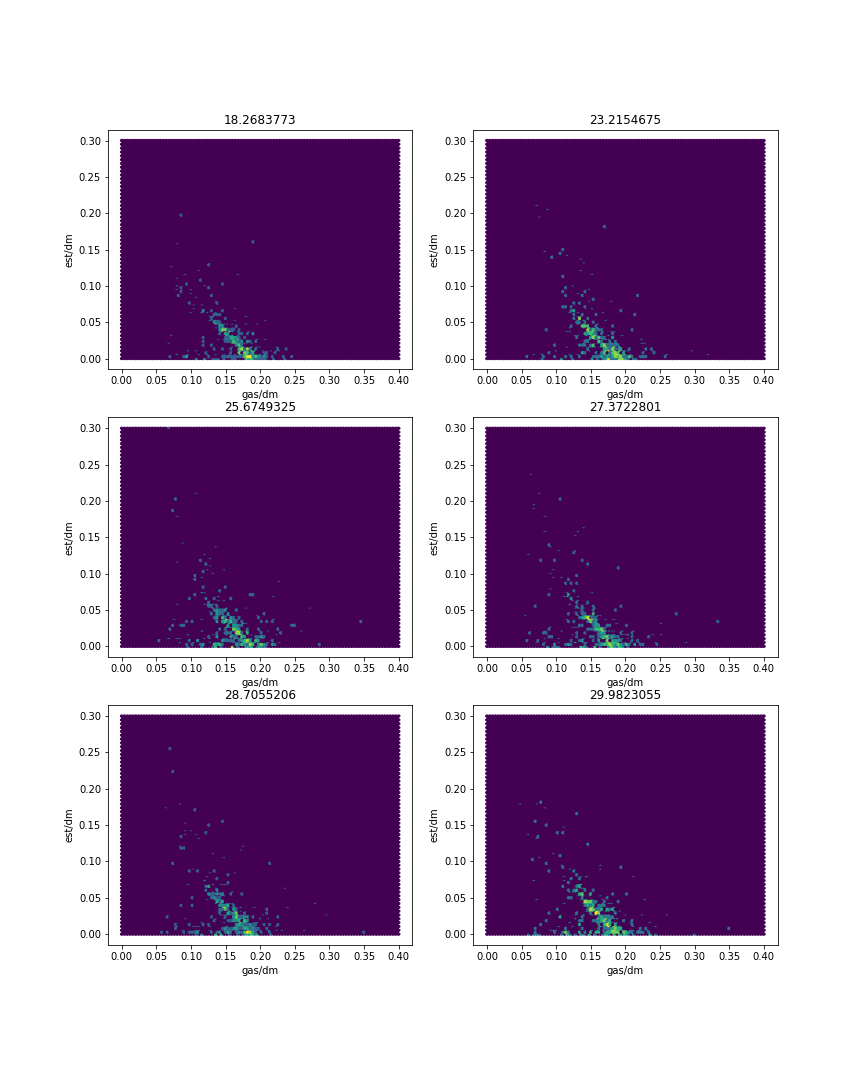
\includegraphics[width=10cm]{Figures/fracciones_R.png}
\decoRule
\caption[asd]{VOID R: esto es en sextiles  }
\label{fig:Electron}
\end{figure}
\begin{figure}[h]
\centering
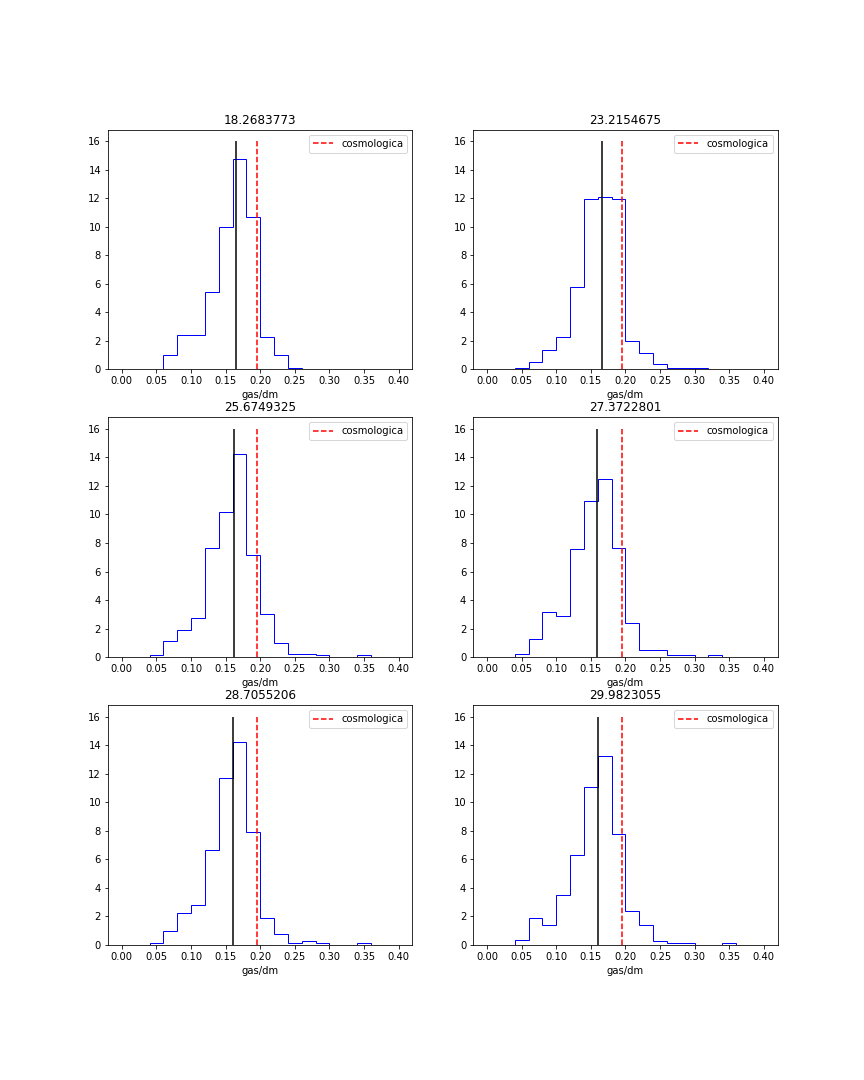
\includegraphics[width=10cm]{Figures/histogramas_R.png}
\decoRule
\caption[asd]{VOID R: SEXTILES  }
\label{fig:Electron}
\end{figure}

\begin{figure}[h]
\centering
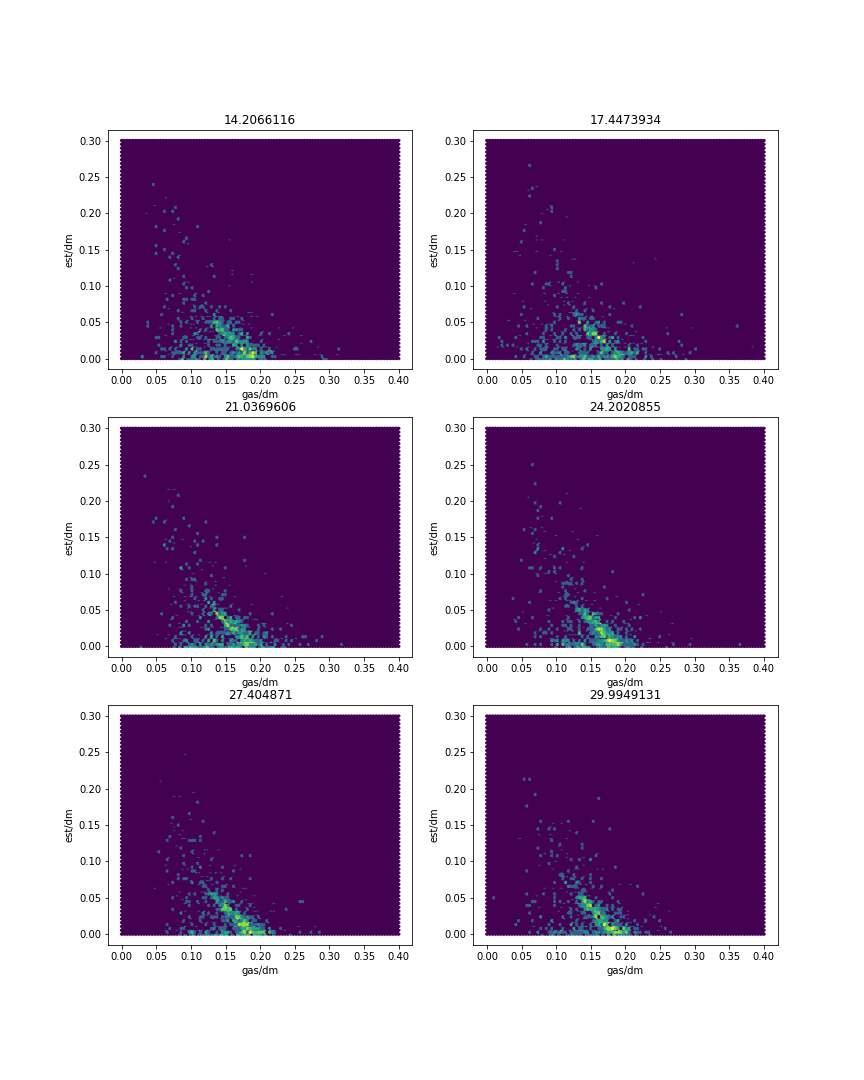
\includegraphics[width=10cm]{Figures/fracciones_S.png}
\decoRule
\caption[asd]{VOID S SEXTILES  }
\label{fig:Electron}
\end{figure}
\begin{figure}[h]
\centering
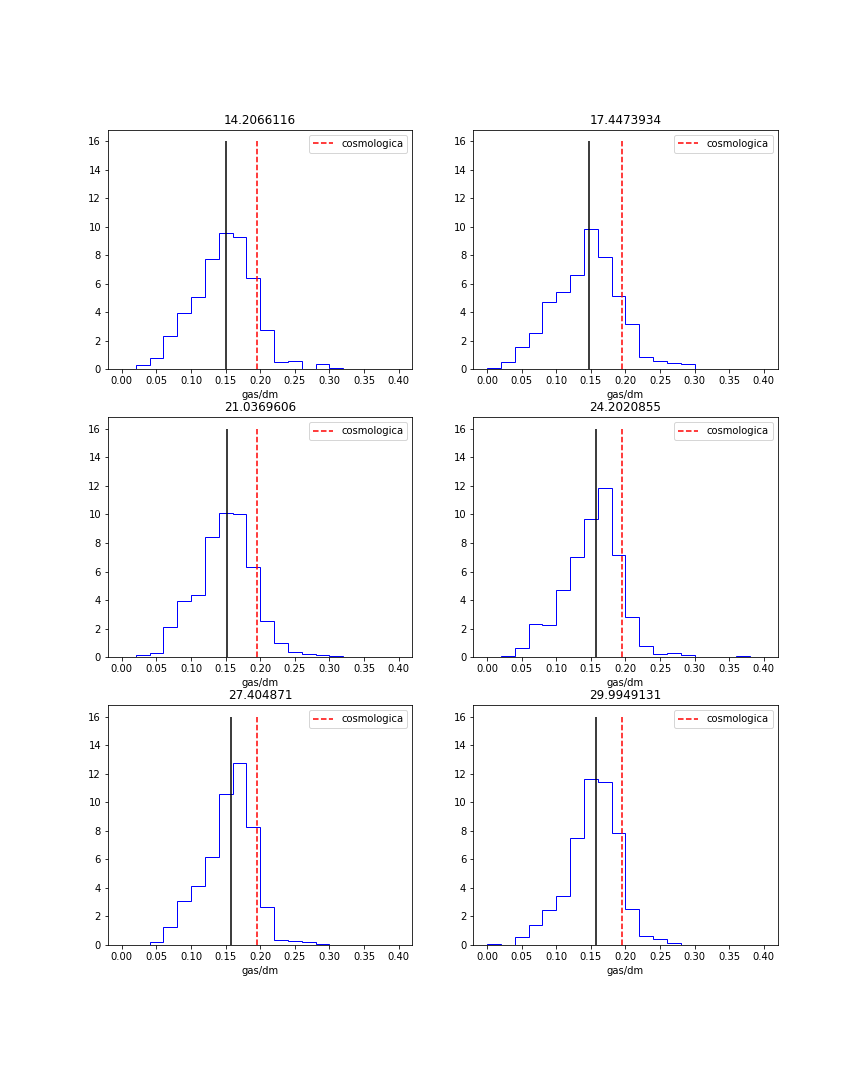
\includegraphics[width=10cm]{Figures/histogramas_S.png}
\decoRule
\caption[asd]{VOID S  SEXTILES}
\label{fig:Electron}
\end{figure}

\begin{figure}[h]
\centering
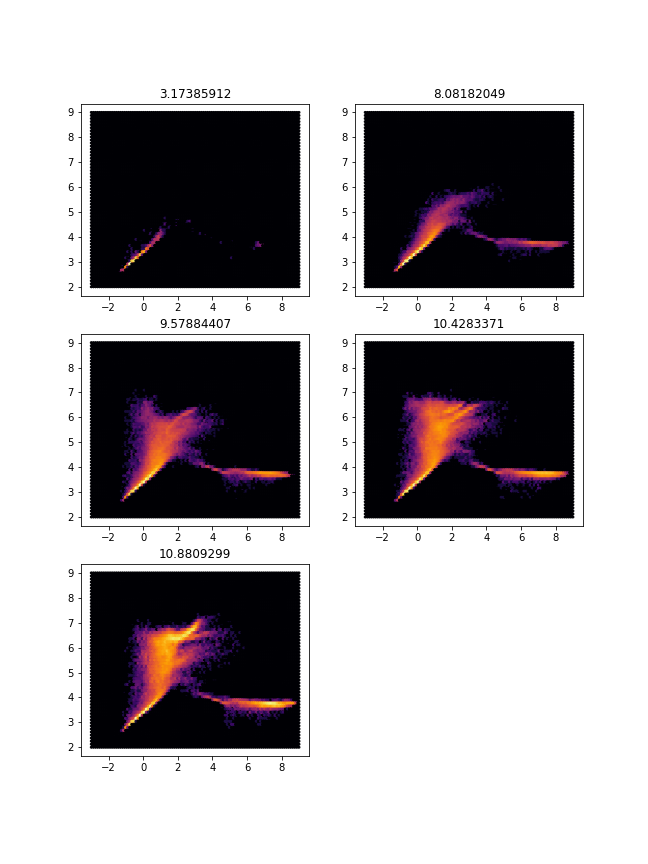
\includegraphics[width=10cm]{Figures/DFprof_S.png}
\decoRule
\caption[asd]{VOID S  estos son intervalos de delta integrada, -1/-0.8; -0.8/-0.6, etc.. hasta 0. El numero de arriba de los plots es la distancia al centro del void.}
\label{fig:Electron}
\end{figure}


\begin{figure}[h]
\centering
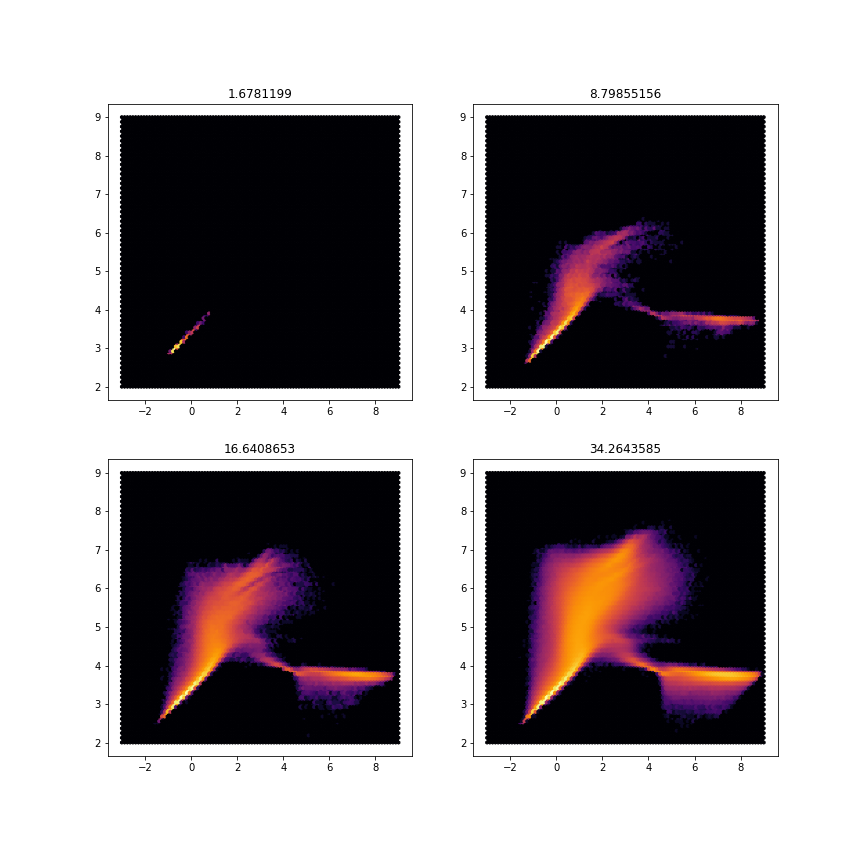
\includegraphics[width=10cm]{Figures/DFprof_R.png}
\decoRule
\caption[asd]{VOID R estos son intervalos de delta integrada, -1/-0.8; -0.8/-0.6, etc.. hasta 0. El numero de arriba de los plots es la distancia al centro del void. }
\label{fig:Electron}
\end{figure}

\begin{figure}[h]
\centering
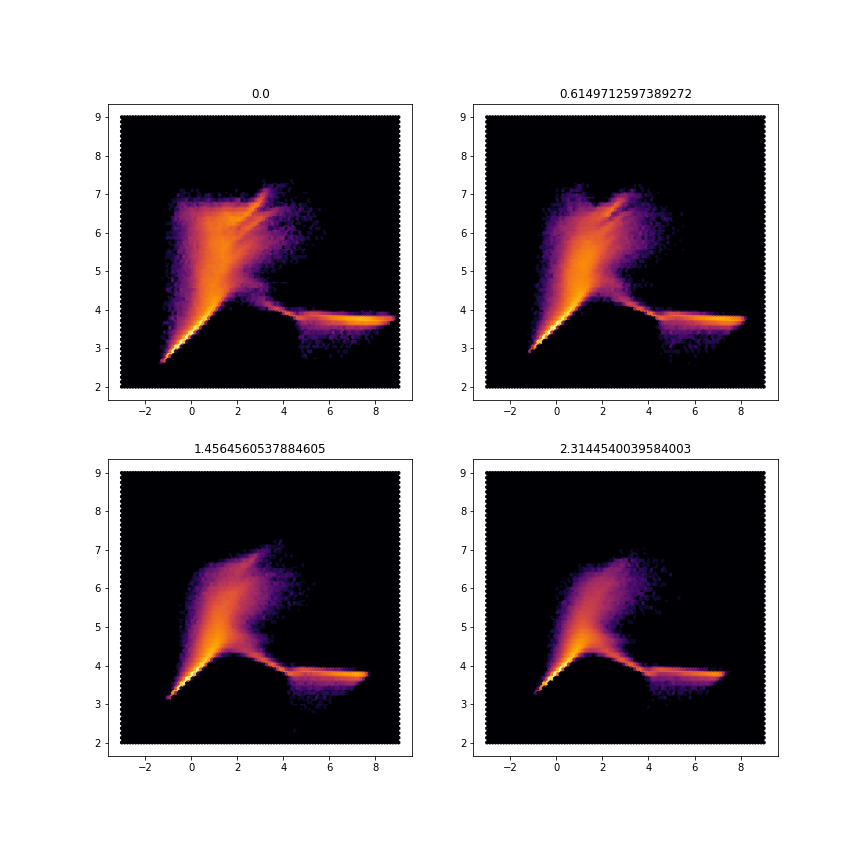
\includegraphics[width=10cm]{Figures/DF_wallS.png}
\decoRule
\caption[asd]{VOID S: esto es entre 5<r<11. El numero de arriba del plot es el redshit  }
\label{fig:Electron}
\end{figure}

\begin{figure}[h]
\centering
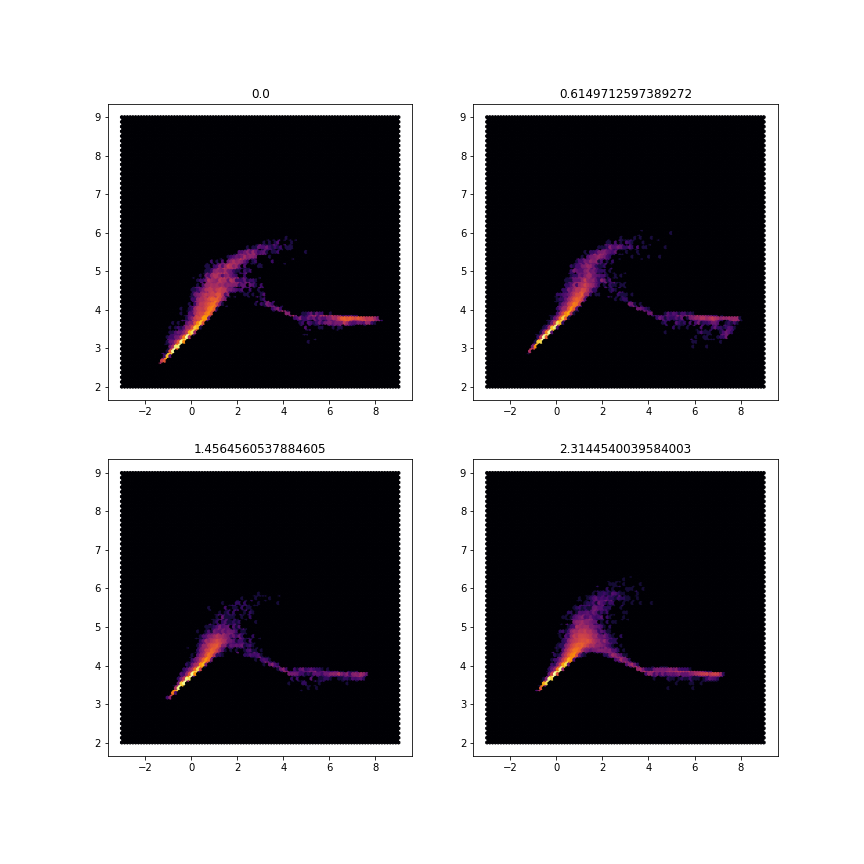
\includegraphics[width=10cm]{Figures/DF_inS.png}
\decoRule
\caption[asd]{VOID S: esto es para r<5  El numero de arriba del plot es el redshit    }
\label{fig:Electron}
\end{figure}

\begin{figure}[h]
\centering
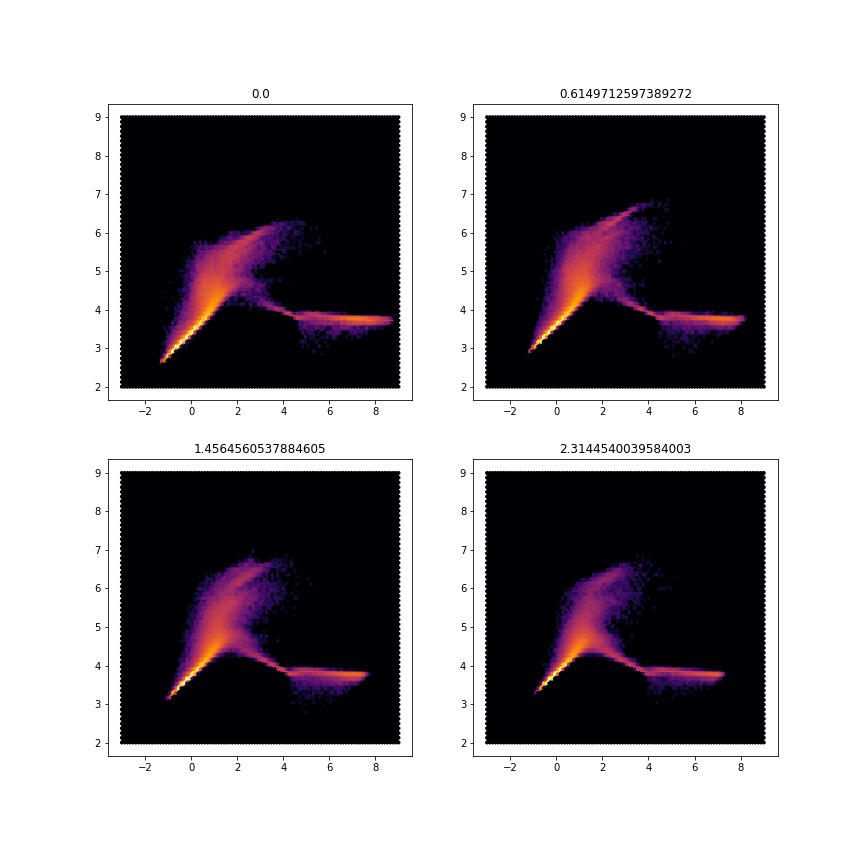
\includegraphics[width=10cm]{Figures/DF_wallR.png}
\decoRule
\caption[asd]{VOID R: esto es entre 5<r<11  El numero de arriba del plot es el redshit   }
\label{fig:Electron}
\end{figure}

\begin{figure}[h]
\centering
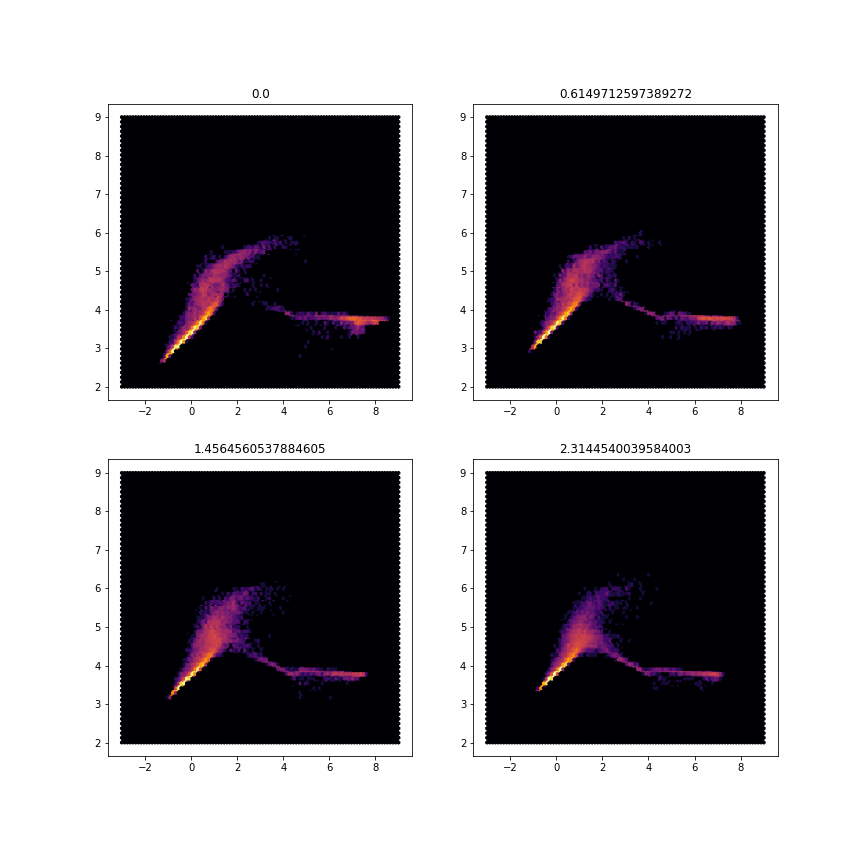
\includegraphics[width=10cm]{Figures/DF_inR.png}
\decoRule
\caption[asd]{VOID R: esto es para r<5  El numero de arriba del plot es el redshit   }
\label{fig:Electron}
\end{figure}

\begin{figure}[h]
\centering
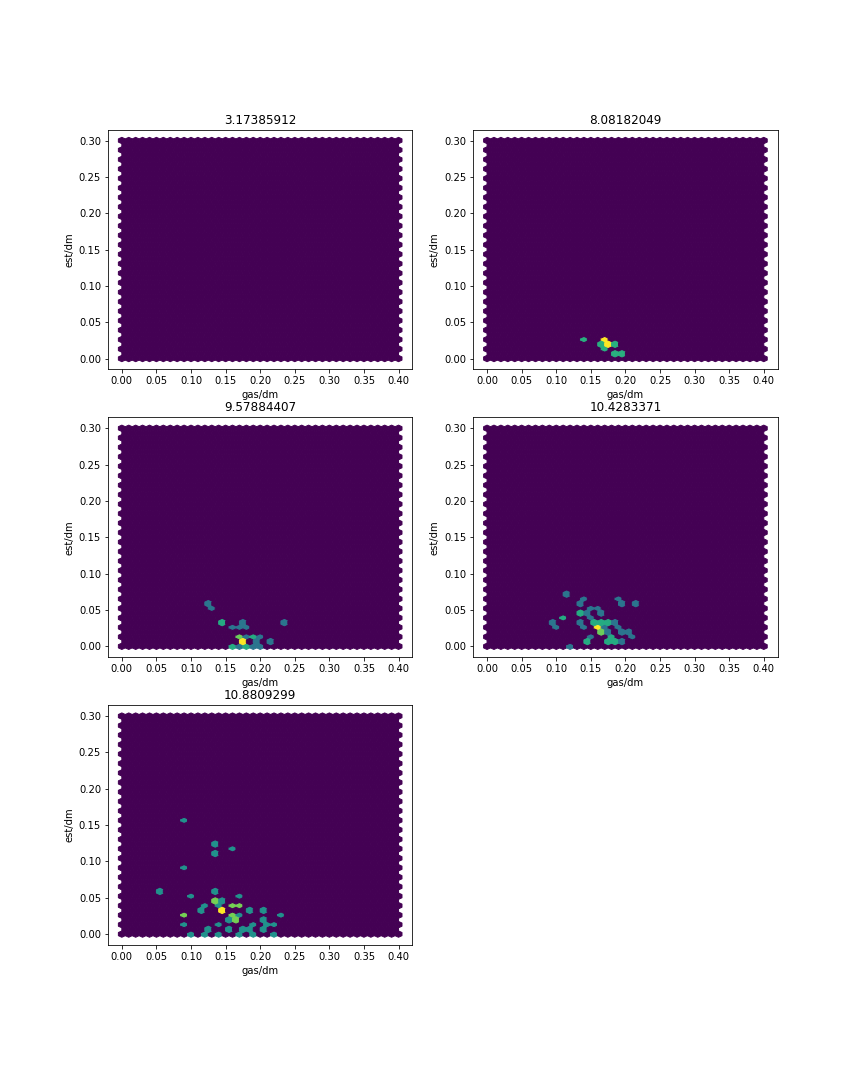
\includegraphics[width=10cm]{Figures/fraccionesDelta_S.png}
\decoRule
\caption[asd]{VOID S, las fracciones son para los halos que tienen estrellas. Cada plot es un intervalo de delta integrada }
\label{fig:Electron}
\end{figure}

\begin{figure}[h]
\centering
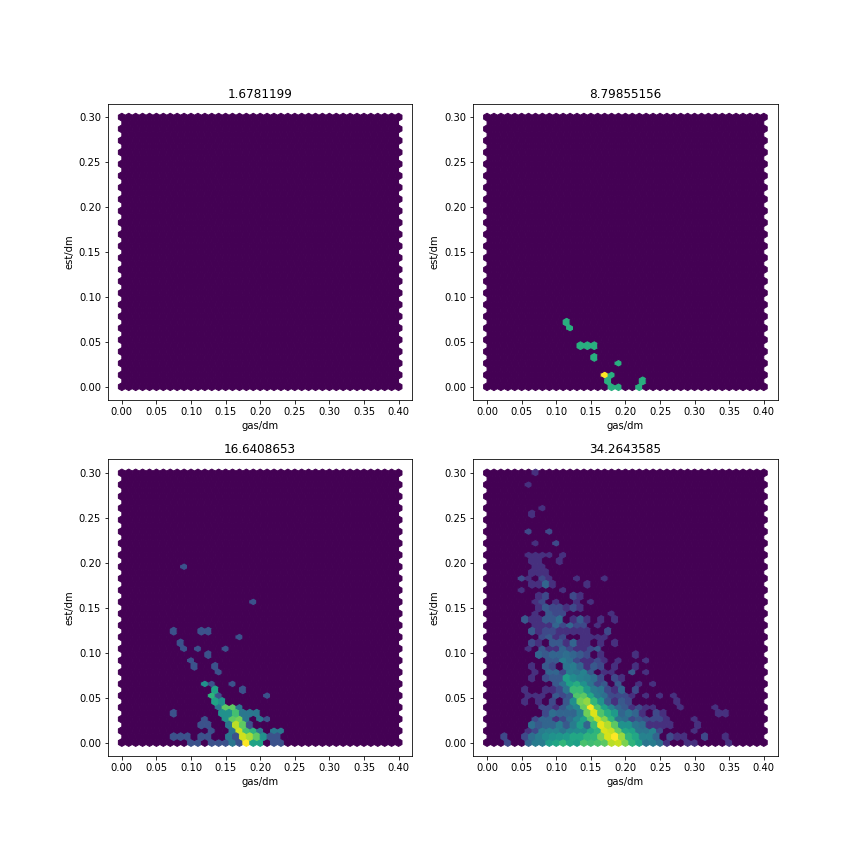
\includegraphics[width=10cm]{Figures/fraccionesDelta_R.png}
\decoRule
\caption[asd]{VOID R: halos con estrellas. Cada plot es un intervalo de delta integrada }
\label{fig:Electron}
\end{figure}

\begin{figure}[h]
\centering
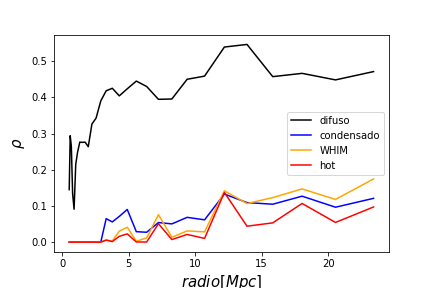
\includegraphics[width=10cm]{Figures/FasesProf_R.png}
\decoRule
\caption[asd]{VOID R. Estos son particulas/vol.  }
\label{fig:Electron}
\end{figure}

\begin{figure}[h]
\centering
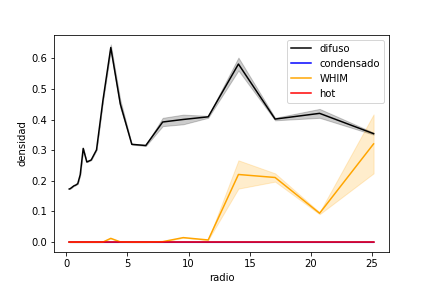
\includegraphics[width=10cm]{Figures/ProfFases_R.png}
\decoRule
\caption[asd]{VOID R: Con jacknife, con 48 realizaciones,500 mediciones y promedios cada 20 }
\label{fig:Electron}
\end{figure}

\begin{figure}[h]
\centering
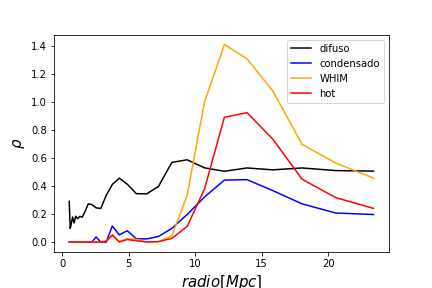
\includegraphics[width=10cm]{Figures/FasesProf_S.png}
\decoRule
\caption[asd]{VOID S , p articulas/volumen}
\label{fig:Electron}
\end{figure}

\begin{figure}[h]
\centering
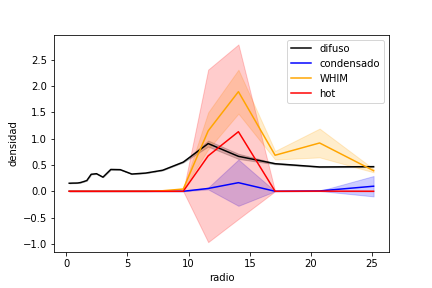
\includegraphics[width=10cm]{Figures/ProfFases_S.png}
\decoRule
\caption[asd]{VOID S: Con jacknife, con 48 realizaciones, 500 mediciones y promedios cada 20. }
\label{fig:Electron}
\end{figure}





\begin{figure}[h]
\centering
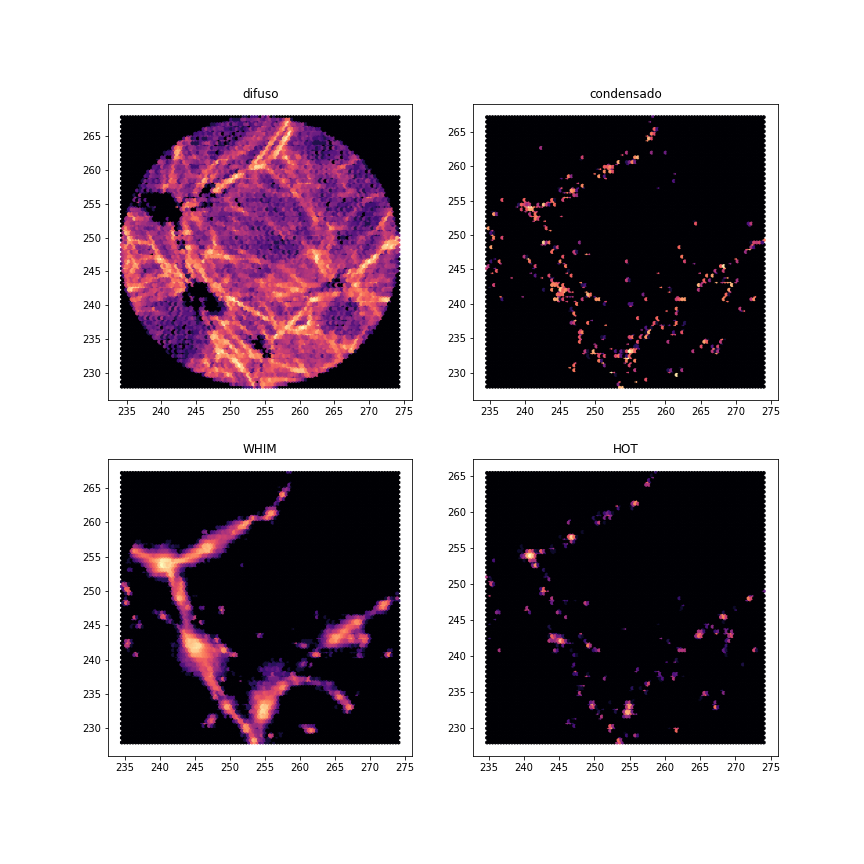
\includegraphics[width=10cm]{Figures/FasesHexbin_S.png}
\decoRule
\caption[asd]{VOID S, es un corte transversal de 4 Mpc de profundidad que pasa por el centro del void }
\label{fig:Electron}
\end{figure}

\begin{figure}[h]
\centering
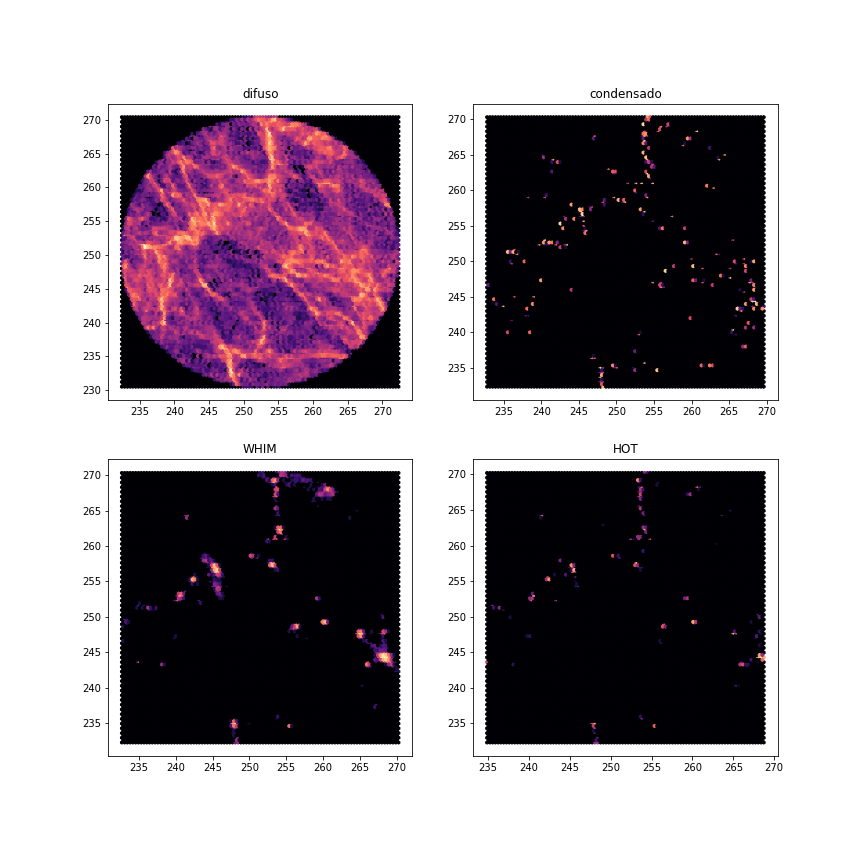
\includegraphics[width=10cm]{Figures/FasesHexbin_R.png}
\decoRule
\caption[asd]{VOID R, es un corte transversal de 4 Mpc de profundidad que pasa por el centro del void }
\label{fig:Electron}
\end{figure}